%============================================================================
% tento soubor pouzijte jako zaklad
% (c) 2008 Michal Bidlo
% E-mail: bidlom AT fit vutbr cz
%============================================================================
% kodovaní: utf-8 (zmena prikazem iconv, recode nebo cstocs)
%----------------------------------------------------------------------------
% zpracování: make, make pdf, make desky, make clean
% připomínky posílejte na e-mail: bidlom AT fit.vutbr.cz
% vim: set syntax=tex encoding=utf-8:
%============================================================================
\documentclass[english,cover]{fitthesis} % odevzdani do wisu - odkazy, na ktere se da klikat
%\documentclass[cover,print]{fitthesis} % pro tisk - na odkazy se neda klikat
%\documentclass[english,print]{fitthesis} % pro tisk - na odkazy se neda klikat
%      \documentclass[english]{fitthesis}
% * Je-li prace psana v anglickem jazyce, je zapotrebi u tridy pouzit 
%   parametr english nasledovne:
%      \documentclass[english]{fitthesis}
% * Neprejete-li si vysazet na prvni strane dokumentu desky, zruste 
%   parametr cover

% zde zvolime kodovani, ve kterem je napsan text prace
% "latin2" pro iso8859-2 nebo "cp1250" pro windows-1250, "utf8" pro "utf-8"
%\usepackage{ucs}
\usepackage[utf8]{inputenc}
\usepackage[T1, IL2]{fontenc}
\usepackage{url}

\DeclareUrlCommand\url{\def\UrlLeft{<}\def\UrlRight{>} \urlstyle{tt}}

%zde muzeme vlozit vlastni balicky
\usepackage{amsmath}
\usepackage{amsthm}
\usepackage{color}
\usepackage{comment}
\usepackage{graphicx}
\usepackage{caption}
\usepackage{subcaption}
\newtheorem{math_def}{Definition}[chapter] % 3. parametr zajisti cislovani "<sekce>.<číslo definice>"
\newcommand{\term}[1]{\emph{#1}}           % novy termin v textu prace
\newcommand{\vars}[1]{{\bold{#1}}}         % matematicke vyrazy - mnozina promennych
\newcommand{\ignore}[1]{}                  % komentar v radku
% znacky rozpracovane prace
\newcommand{\todo}[1]{{\color{red} #1}}
\newcommand{\uncertain}[1]{{\color{blue} #1}}
\newcommand{\note}[1]{{\color{green} #1}}

% =======================================================================
% balíček "hyperref" vytváří klikací odkazy v pdf, pokud tedy použijeme pdflatex
% problém je, že balíček hyperref musí být uveden jako poslední, takže nemůže
% být v šabloně
\ifWis
\ifx\pdfoutput\undefined % nejedeme pod pdflatexem
\else
  \usepackage{color}
  \usepackage[unicode,colorlinks,hyperindex,plainpages=false,pdftex]{hyperref}
  \definecolor{links}{rgb}{0.4,0.5,0}
  \definecolor{anchors}{rgb}{1,0,0}
  \def\AnchorColor{anchors}
  \def\LinkColor{links}
  \def\pdfBorderAttrs{/Border [0 0 0] }  % bez okrajů kolem odkazů
  \pdfcompresslevel=9
\fi
\fi

%Informace o praci/projektu
%---------------------------------------------------------------------------
\projectinfo{
  %Prace
  project=SP,            %typ prace BP/SP/DP/DR
  year=2012,             %rok
  date=\today,          %datum odevzdani
  %Nazev prace
  title.cs={Aplikace Bayesovských sítí},  %nazev prace v cestine
  title.en={Bayesian Networks Applications}, %nazev prace v anglictine
  %Autor
  author={David Chaloupka},   %jmeno prijmeni autora
  author.title.p=Bc., %titul pred jmenem (nepovinne)
  %author.title.a=PhD, %titul za jmenem (nepovinne)
  %Ustav
  department=UITS, % doplnte prislusnou zkratku: UPSY/UIFS/UITS/UPGM
  %Skolitel
  supervisor=František V. Zbořil, %jmeno prijmeni skolitele
  supervisor.title.p=doc.~Ing.,   %titul pred jmenem (nepovinne)
  supervisor.title.a={CSc.},    %titul za jmenem (nepovinne)
  %Klicova slova, abstrakty, prohlaseni a podekovani je mozne definovat 
  %bud pomoci nasledujicich parametru nebo pomoci vyhrazenych maker (viz dale)
  %===========================================================================
  %Klicova slova
  keywords.cs={Bayesovská síť, pravděpodobnost, inference, učení struktury.}, %klicova slova v ceskem jazyce
  keywords.en={Bayesian network, probability, inference, structure learning.}, %klicova slova v anglickem jazyce
  %Abstract
  abstract.cs={Výtah (abstrakt) práce v českém jazyce.}, % abstrakt v ceskem jazyce
  abstract.en={Výtah (abstrakt) práce v anglickém jazyce.}, % abstrakt v anglickem jazyce
  %Prohlaseni
  declaration={Prohlašuji, že jsem tento semestrální projekt vypracoval samostatně pod vedením pana doc.~Ing.~Františka V. Zbořila,~CSc.},
  %Podekovani (nepovinne)
  acknowledgment={Zde je možné uvést poděkování vedoucímu práce a těm, kteří poskytli odbornou pomoc.} % nepovinne
}

%Abstrakt (cesky, anglicky)
%\abstract[cs]{Do tohoto odstavce bude zapsán výtah (abstrakt) práce v českém jazyce.}
%\abstract[en]{Do tohoto odstavce bude zapsán výtah (abstrakt) práce v anglickém jazyce.}

%Klicova slova (cesky, anglicky)
%\keywords[cs]{Sem budou zapsána jednotlivá klíčová slova v českém jazyce, oddělená čárkami.}
%\keywords[en]{Sem budou zapsána jednotlivá klíčová slova v anglickém jazyce, oddělená čárkami.}

%Prohlaseni
%\declaration{Prohlašuji, že jsem tuto bakalářskou práci vypracoval samostatně pod vedením pana X...
%Další informace mi poskytli...
%Uvedl jsem všechny literární prameny a publikace, ze kterých jsem čerpal.}

%Podekovani (nepovinne)
%\acknowledgment{V této sekci je možno uvést poděkování vedoucímu práce a těm, kteří poskytli odbornou pomoc
%(externí zadavatel, konzultant, apod.).}

\begin{document}
  % Vysazeni titulnich stran
  % ----------------------------------------------
  \maketitle
  % Obsah
  % ----------------------------------------------
  \tableofcontents
  
  % Seznam obrazku a tabulek (pokud prace obsahuje velke mnozstvi obrazku, tak se to hodi)
  % \listoffigures
  % \listoftables 

  % Text prace
  % ----------------------------------------------
  \input{obsah} % viz. obsah.tex

  % Pouzita literatura
  % ----------------------------------------------
\ifczech
  \bibliographystyle{czechiso}
\else 
  \bibliographystyle{plain}
%  \bibliographystyle{alpha}
\fi
  \begin{flushleft}
  \bibliography{literatura} % viz. literatura.bib
  \end{flushleft}
  \appendix
  
  \chapter{Notation overview}\label{ch:appendix_notation}
This chapter presents listing of the mathematical notation used in this thesis:

\bigskip
\begin{tabular}{ll}
	$X$ & Capital letter denotes a random variable.\\
	&\\
	$x$ & Lowercase letter denotes a concrete instantiation of the variable $X$.\\
	&\\
	$\vars{X}$ & Capital bold letter denotes a set of random variables.\\
	&\\
	$\vars{x}$ & Lowercase bold letter denotes an instantiation of all variables in the set $\vars{X}$.\\
	&\\
	$val(\vars{X})$ & Set of all possible instantiations of variables $\vars{X}$.\\
	&\\
	$Parents(X)$ & Set of parent variables of variable $X$ in a Bayesian network.\\
	&\\
	$parents(X)$ & Instantiation of parent variables of variable $X$ in a Bayesian network.\\
	&\\
	$Children(X)$ & Set of child variables of variable $X$ in a Bayesian network.\\
	&\\
	$children(X)$ & Instantiation of child variables of variable $X$ in a Bayesian network.\\
	&\\
	$N_x$ & Number of samples of a dataset for which variable $X$ has the value $x$.\\
	&\\
	$N_{x,\vars{pa}}$ & Number of samples of a dataset for which $X$ has the value $x$ and variables\\
	                  & $Parents(X)$ have the value $\vars{pa}$.\\
	&\\
	$\sum_\vars{X} (\dots)$ & Summation over instantiations $\vars{x}$ of the variables $\vars{X}$.\\
	&\\
	$P(\vars{X})$ & Probability distribution over variables $\vars{X}$.\\
	&\\
	$P(\vars{x})$ & Probability of variables $\vars{X}$ having the concrete instantiation $\vars{x}$.\\
\end{tabular}










\chapter{CD Content}\label{ch:appendix_cd_content}
Content of the enclosed CD is organized into the following directories:
\begin{itemize}
    \item \srccode{1-benchmarks/}: Network \srccode{.net} files, datasets and measurements related to the first practical application.
    \item \srccode{2-crime/}: Vector images of the final three networks that resulted from the analysis of criminality. Also contains the original dataset, its discretized version, networks learnt during the feature elimination process and records of analysis of the crime impact factor.
    \item \srccode{3-spam/}: Datasets (the original dataset, its discretized version, train and test sets for holdout testing and for 5-fold cross-validation). Also contains measurement records and figures.
    \item \srccode{program/}: Program source codes compilable using the \emph{ant} build tool and also runnable compiled version in \srccode{program/bin-precompiled}.
    \item \srccode{text/}:  {\LaTeX} sources of this thesis, including all figures.
\end{itemize} 





\chapter{Crime analysis\,--\,final networks}\label{ch:appendix_crime_net}
This chapter contains the three networks that are result of the crime analysis performed in Section~\ref{ch:practical_crime}. Because of their size, each network is on its own A3 page. If you have trouble reading variable names in the printed version please see the electronic version of this thesis or the original figures on the encolsed CD within the directory \srccode{2-crime/final networks/}.


\begin{hugepage}
\pdfpagewidth=2\pdfpagewidth
\begin{figure}[h]
    \centering
    \vspace*{-2.5cm}
    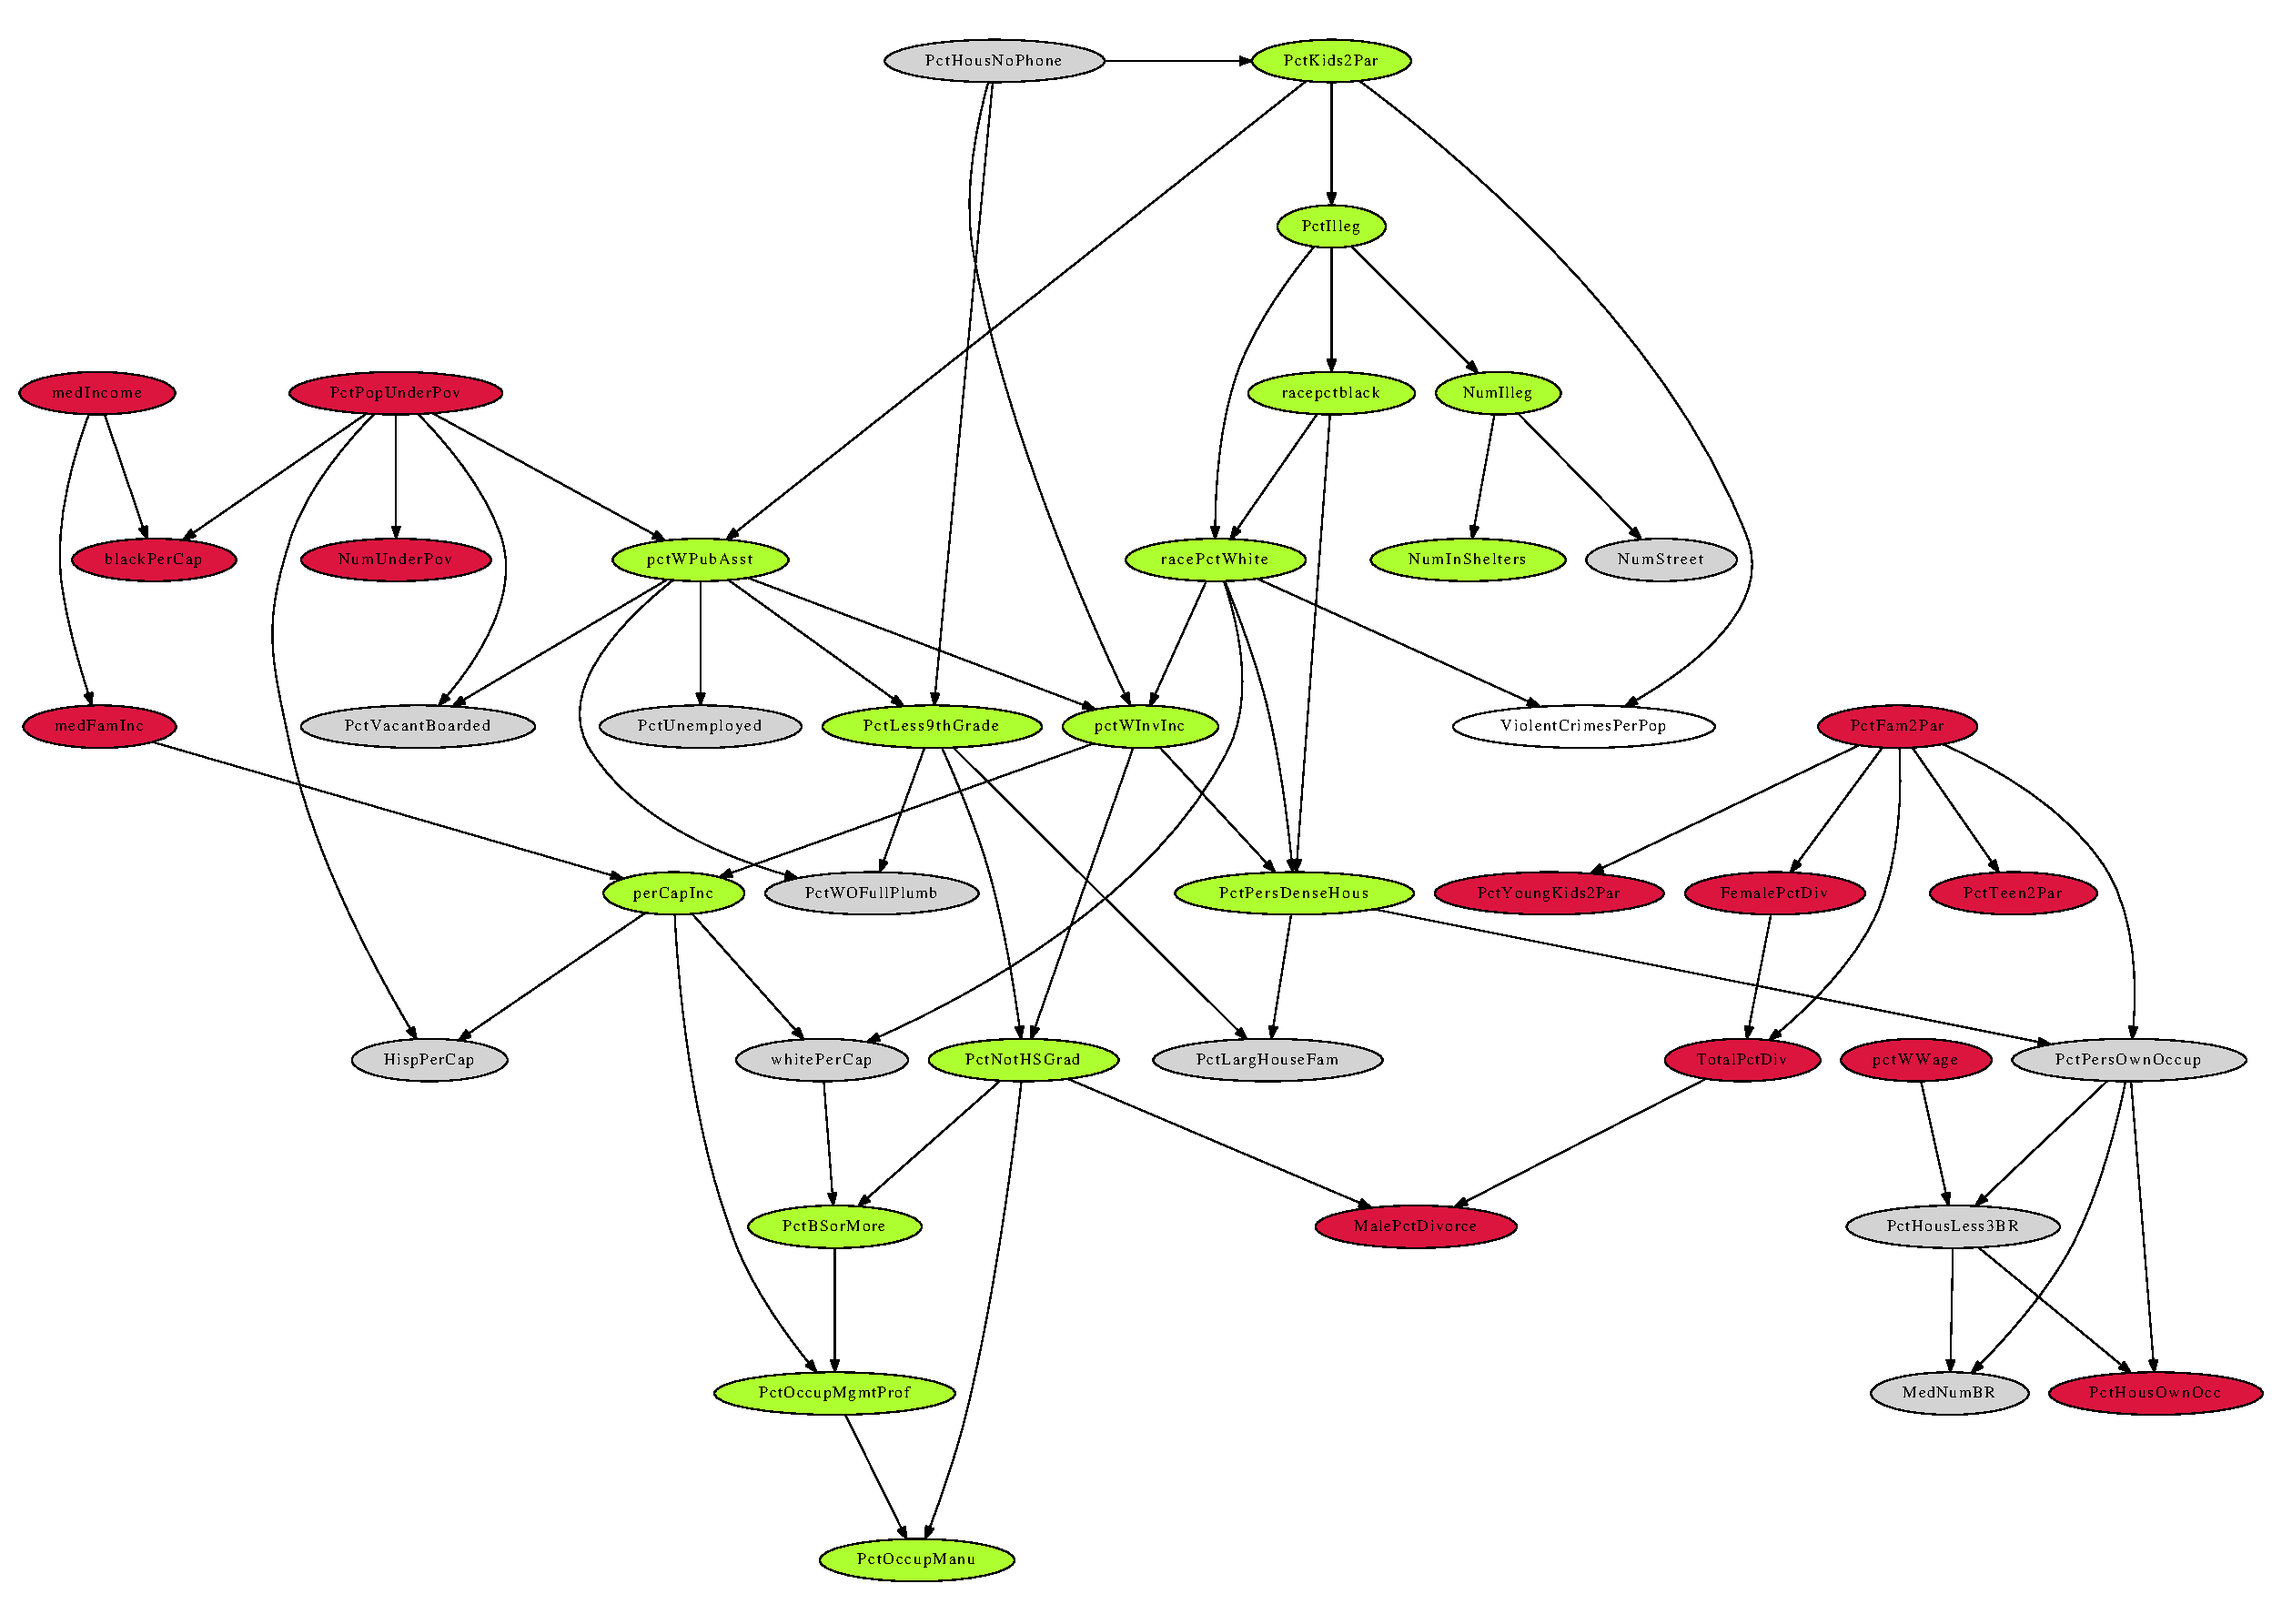
\includegraphics[scale=0.834]{fig/top-40_intersection_tolerance-1}
    \caption{Bayesian network for crime containing top 40 attributes with the highest crime impact factor.
    \\Legend: Green variables influence the $ViolentCrimesPerPop$ the same way as in the network with all 100 features. Influence of red variables is significantly different and therefore these variables shouldn't be considered.}
    \label{fig:crime_net_top40}
\end{figure}
\end{hugepage}

\begin{hugepage}
\pdfpagewidth=2\pdfpagewidth
\begin{figure}[h]
    \centering
    \vspace*{-2.5cm}
    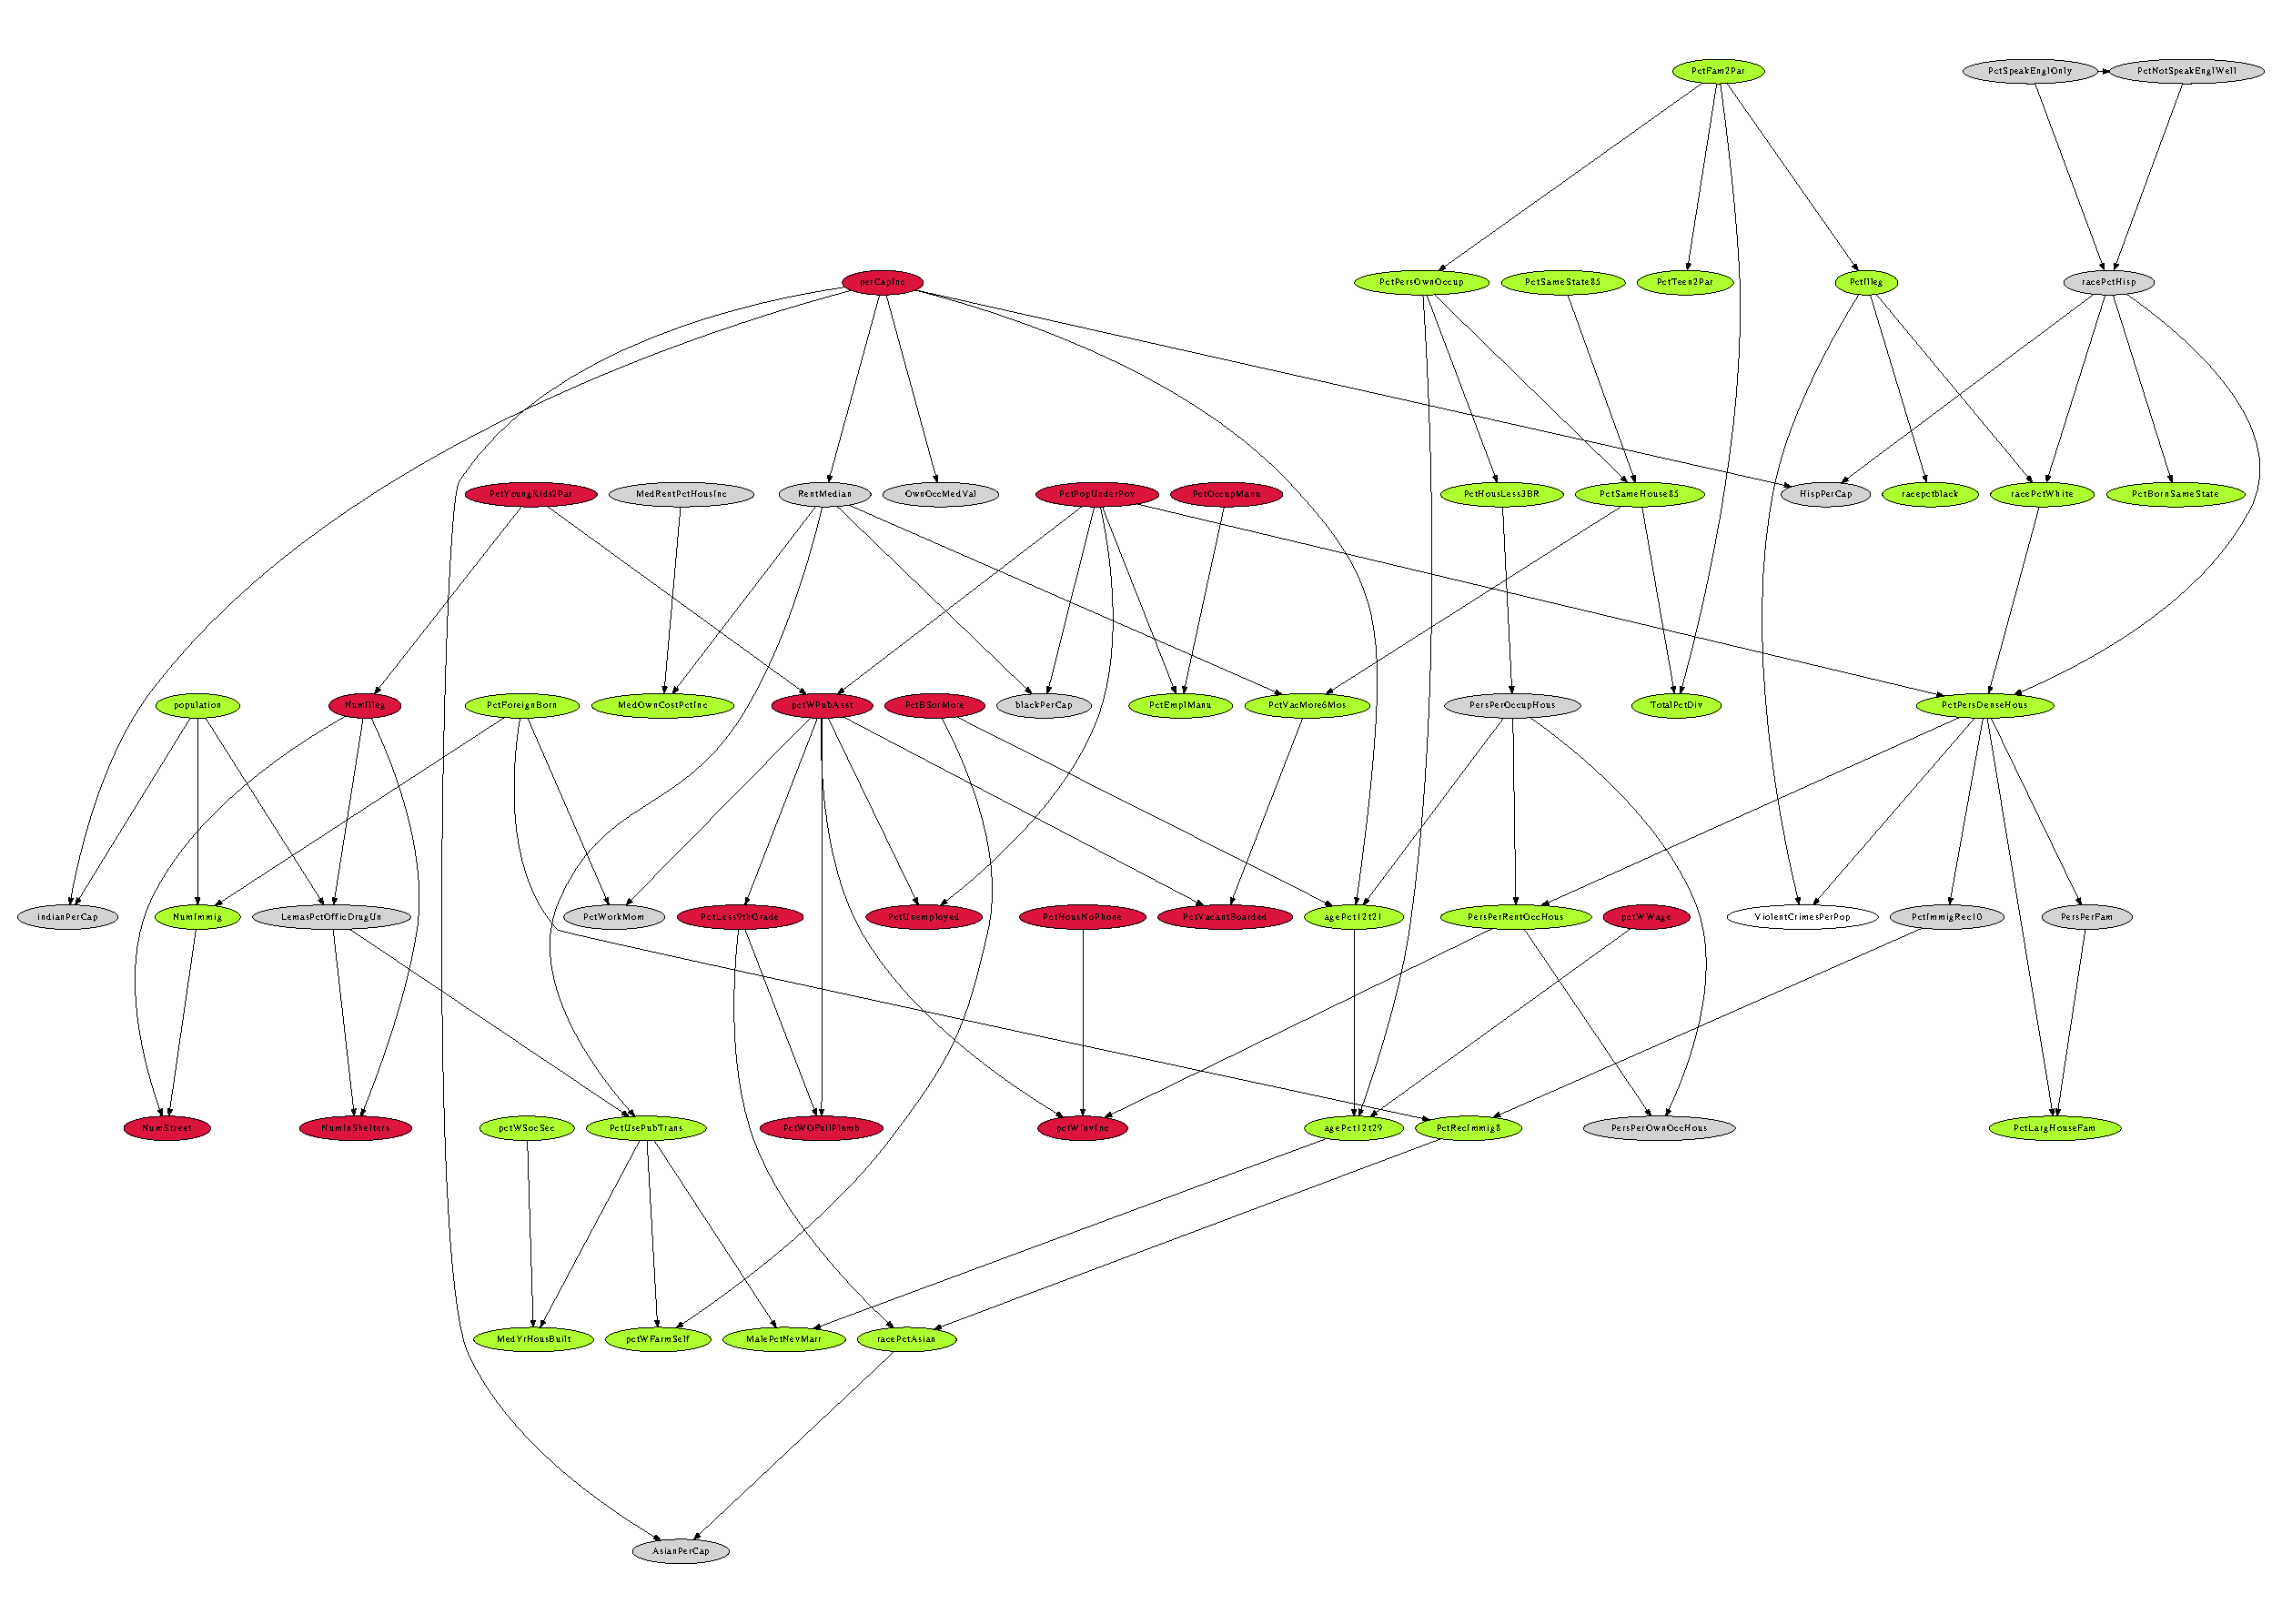
\includegraphics[scale=0.83]{fig/round-3_intersection_tolerance-1}
    \caption{Final Bayesian network for crime after three rounds of iterative elimination of similar variables.
    \\Legend: Green variables influence the $ViolentCrimesPerPop$ the same way as in the network with all 100 features. Influence of red variables is significantly different and therefore these variables shouldn't be considered.}
    \label{fig:crime_net_round3}
\end{figure}
\end{hugepage}

\begin{hugepage}
\pdfpagewidth=2\pdfpagewidth
\begin{figure}[h]
    \centering
    \vspace*{-2.5cm}
    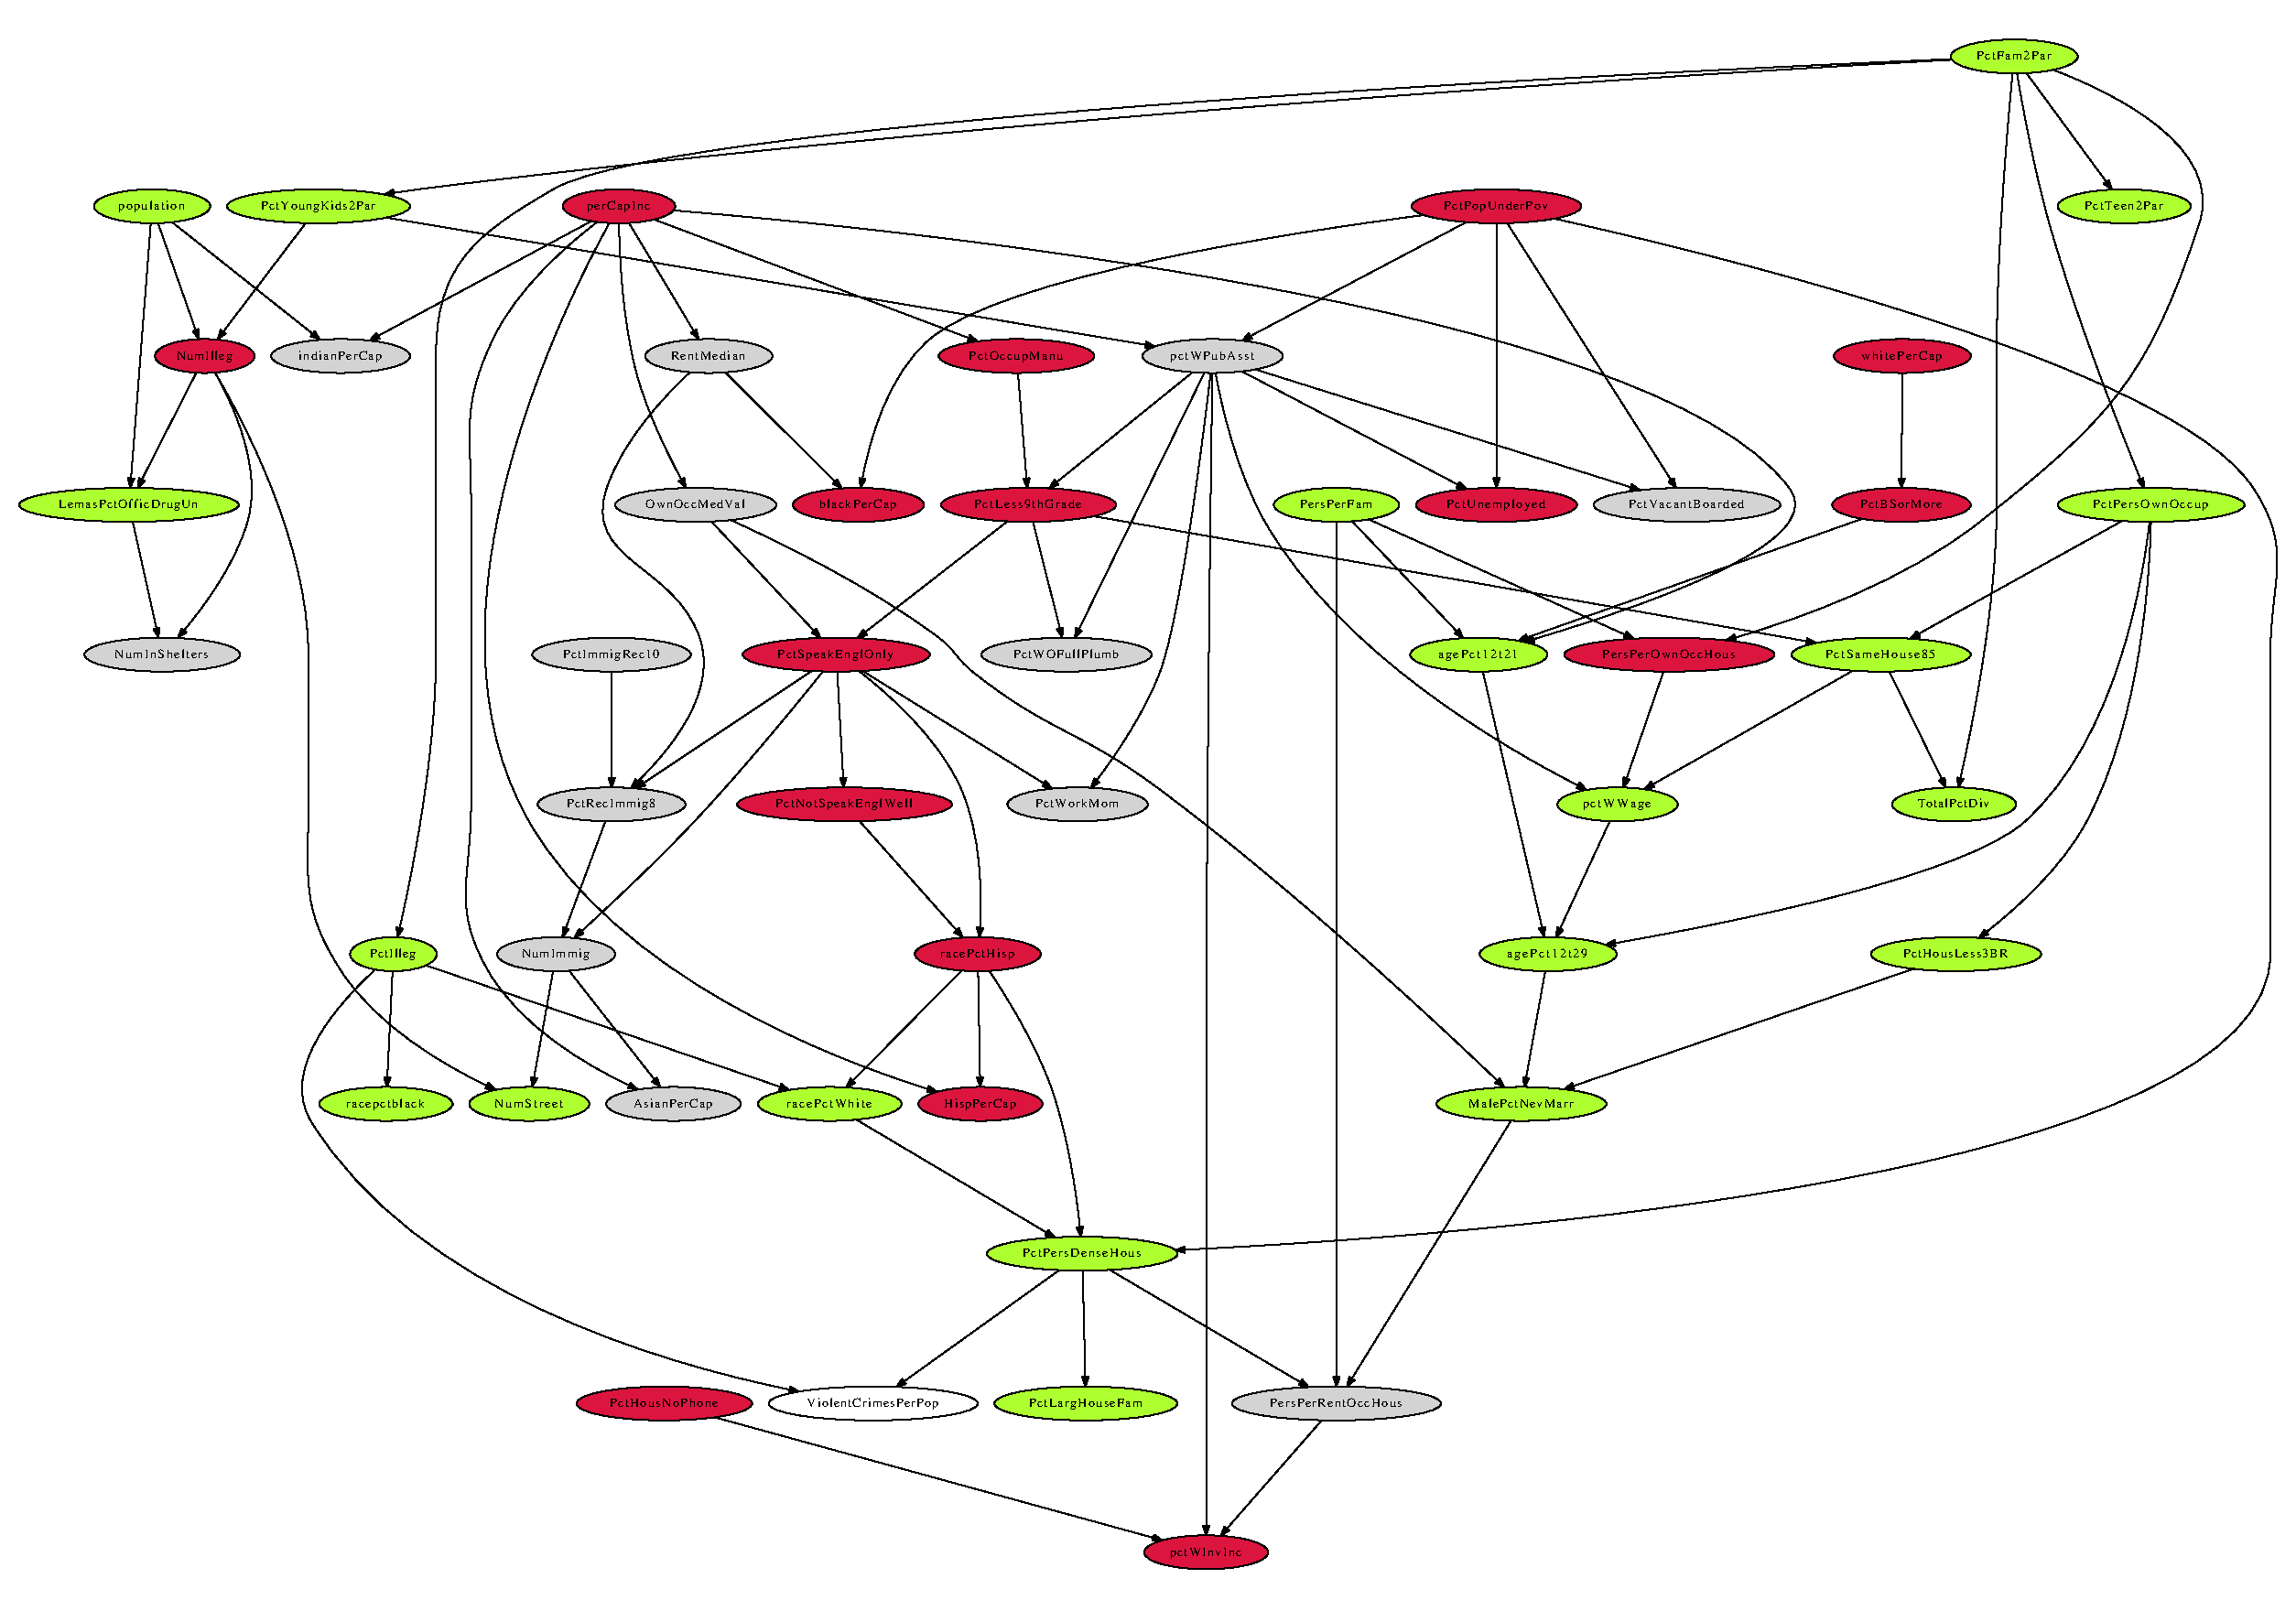
\includegraphics[scale=0.83]{fig/round-4_intersection_tolerance-1}
    \caption{Final Bayesian network for crime after three rounds of iterative elimination of similar variables and additional removal of variables whose crime impact factor is less than 0.07.
    \\Legend: Green variables influence the $ViolentCrimesPerPop$ the same way as in the network with all 100 features. Influence of red variables is significantly different and therefore these variables shouldn't be considered.}
    \label{fig:crime_net_round4}
\end{figure}
\end{hugepage}


 % viz. prilohy.tex
\end{document}
